\chapter{Conception}
\label{chap:conception}

Ce chapitre présente la conception des deux solutions. Pour le \ac{CTAA}, nous décrivons l'architecture du module de traçabilité, son principe de fonctionnement, la structure des codes et l'algorithme qui les interprète, les échanges entre ses composants et le modèle de données sur lequel il s'appuie. Pour Pharmaghreb, nous détaillons l'architecture matérielle du module d'acquisition, le choix des composants, le câblage, le protocole de communication avec la balance et la logique du programme embarqué.

%=============================================================
\section{Conception du module de traçabilité (CTAA)}
%=============================================================

\subsection{Architecture logicielle}

Le module de traçabilité est intégré au \ac{LIMS}. Il repose sur une architecture en trois niveaux (figure~\ref{fig:architecture-tracabilite}) :
\begin{itemize}
    \item \textbf{le niveau présentation} (\ac{HTML}, CSS et JavaScript) s'exécute dans le navigateur. Il reçoit le contenu lu par la douchette, qui se comporte comme un clavier, et l'envoie au serveur par une requête \ac{AJAX}, c'est-à-dire sans recharger la page ;
    \item \textbf{le niveau application} (\ac{PHP}) reçoit la requête, identifie le type de code, construit et exécute les requêtes \ac{SQL}, puis renvoie le résultat au format \ac{JSON} \citep{php} ;
    \item \textbf{le niveau données} est la base PostgreSQL du \ac{LIMS}, qui contient les demandes, les échantillons, les réceptions, les préparations, les lots et les utilisateurs \citep{postgresql}.
\end{itemize}

\begin{figure}[H]
\centering
\begin{tikzpicture}
  \node[bloc=2.6cm] (douchette) at (0,3.0) {\textbf{Douchette}\\{\scriptsize codes QR et codes-barres}};
  \node[bloc=3.0cm, minimum height=2.8cm] (client) at (0,0)
       {\textbf{Navigateur}\\[3pt] HTML / CSS\\ JavaScript\\ {\scriptsize affichage dynamique}};
  \node[blocvert=3.4cm, minimum height=2.8cm] (srv) at (5.4,0)
       {\textbf{Serveur web}\\[3pt] Back-end PHP\\ {\scriptsize identification du code,\\ requêtes SQL,\\ mise en forme JSON}};
  \node[blocorange=3.0cm, minimum height=2.8cm] (bd) at (10.6,0)
       {\textbf{PostgreSQL}\\[3pt] Base du LIMS\\ {\scriptsize réceptions, préparations,\\ échantillons, lots,\\ utilisateurs}};
  \draw[fleche] (douchette) -- node[right, etiq] {chaîne lue\\(émulation clavier)} (client);
  \draw[fleche] ([yshift=5mm]client.east) -- node[above, etiq] {requête AJAX\\(HTTP)} ([yshift=5mm]srv.west);
  \draw[fleche] ([yshift=-5mm]srv.west) -- node[below, etiq] {réponse\\JSON} ([yshift=-5mm]client.east);
  \draw[fleche] ([yshift=5mm]srv.east) -- node[above, etiq] {requêtes\\SQL} ([yshift=5mm]bd.west);
  \draw[fleche] ([yshift=-5mm]bd.west) -- node[below, etiq] {lignes de\\résultat} ([yshift=-5mm]srv.east);
  \node[etiq, font=\small\bfseries] at (0,-2.0)    {Présentation};
  \node[etiq, font=\small\bfseries] at (5.4,-2.0)  {Application};
  \node[etiq, font=\small\bfseries] at (10.6,-2.0) {Données};
\end{tikzpicture}
\caption{Architecture en trois niveaux du module de traçabilité.}
\label{fig:architecture-tracabilite}
\end{figure}

Cette séparation présente trois avantages : l'interface reste réactive, car seules les données utiles transitent entre le navigateur et le serveur ; la logique d'interprétation des codes est centralisée côté serveur ; enfin, l'ajout d'un nouveau type de code ne modifie que le niveau application.

\subsection{Principe de fonctionnement}

Le module donne un accès immédiat aux informations liées aux opérations du laboratoire. Il propose deux modes de recherche, sélectionnés par l'utilisateur :
\begin{itemize}
    \item \textbf{la recherche par code} : l'utilisateur scanne l'étiquette d'un élément géré par le \ac{LIMS}. Dans le module de gestion des demandes, les étiquettes d'échantillons portent un code \ac{QR}, généré par le bouton « Gén. étiquette » de la demande ; dans les autres modules (réceptions, préparations, stocks), les étiquettes portent pour l'instant un code-barres. La douchette lit indifféremment les deux et transmet leur contenu sous forme de chaîne de caractères ;
    \item \textbf{la recherche par numéro de série} : l'utilisateur saisit ou scanne un numéro de série ou de lot (par exemple celui d'un réactif) afin de retrouver toutes les réceptions qui le concernent.
\end{itemize}

Le traitement se déroule ensuite en quatre étapes : \textbf{lecture} du code, \textbf{identification} de son type, \textbf{interrogation} de la base de données et \textbf{affichage} du résultat ou d'un message d'erreur. Les sections suivantes détaillent ces étapes.

\subsection{Structure des codes et règles d'identification}

Le contenu d'un code est organisé autour du séparateur «~\texttt{\#}~». Le serveur découpe la chaîne en éléments et déduit le type de code d'après leur nombre et certaines valeurs (tableau~\ref{tab:structure-qr}).

\begin{table}[H]
\centering
\renewcommand{\arraystretch}{1.3}
\begin{tabularx}{\textwidth}{|p{6.8cm}|Y|}
\hline
\enteteligne \entete{Contenu du code} & \entete{Interprétation} \\ \hline
Sept éléments, le troisième vaut «~\texttt{CTA}~» & Code de préparation \\ \hline
Sept éléments, le troisième est différent de «~\texttt{CTA}~» & Code de réception \\ \hline
Deux éléments & Analyse complémentaire (présence d'une date) pour déterminer le processus associé \\ \hline
Autre structure & Code incorrect : message d'erreur \\ \hline
\end{tabularx}
\caption{Règles d'identification des codes par le module de traçabilité.}
\label{tab:structure-qr}
\end{table}

Le tableau~\ref{tab:exemple-code} décompose, à titre d'exemple, le code de préparation \texttt{test\#dev\#CTA\#260808\#100\#2026-08-08\#2206214830101} utilisé lors des tests.

% À VÉRIFIER : signification exacte des éléments 1, 2 et 5.
\begin{table}[H]
\centering
\renewcommand{\arraystretch}{1.25}
\begin{tabular}{|c|l|l|}
\hline
\enteteligne \entete{Position} & \entete{Valeur} & \entete{Signification} \\ \hline
1--2 & \texttt{test}, \texttt{dev} & Désignation du produit préparé \\ \hline
3 & \texttt{CTA} & Marqueur d'un code de préparation \\ \hline
4 & \texttt{260808} & Numéro de lot \\ \hline
5 & \texttt{100} & Quantité conditionnée \\ \hline
6 & \texttt{2026-08-08} & Date de préparation \\ \hline
7 & \texttt{2206214830101} & Numéro d'étiquette \\ \hline
\end{tabular}
\caption{Exemple de décomposition d'un code de préparation.}
\label{tab:exemple-code}
\end{table}

La figure~\ref{fig:algo-identification} présente l'algorithme d'identification exécuté par le serveur.

\begin{figure}[H]
\centering
\begin{tikzpicture}[
    decision/.append style={text width=2.2cm, font=\scriptsize},
    bloc/.append style={font=\scriptsize}]
  \node[debutfin] (start) at (0,0) {Code reçu};
  \node[decision] (mode) at (0,-1.7) {Mode de recherche ?};
  \node[bloc=2.8cm] (serie) at (-4.6,-1.7) {Rechercher les réceptions du lot};
  \node[bloc=2.8cm] (split) at (0,-3.4) {Découper la chaîne selon «~\#~»};
  \node[decision] (n7) at (0,-5.1) {Sept éléments ?};
  \node[decision] (cta) at (-4.6,-5.1) {3\textsuperscript{e} élément = CTA ?};
  \node[bloc=2.2cm] (prep) at (-6.4,-7.0) {Préparation};
  \node[bloc=2.2cm] (recep) at (-2.8,-7.0) {Réception};
  \node[decision] (n2) at (0,-7.0) {Deux éléments ?};
  \node[bloc=2.8cm] (date) at (4.6,-7.0) {Analyse complémentaire (date)};
  \node[blocorange=2.8cm] (err) at (0,-9.0) {Code incorrect :\\message d'erreur};
  \node[bloc=3.2cm] (sql) at (-4.6,-9.0) {Requête SQL selon le type};
  \node[decision] (vide) at (-4.6,-10.9) {Résultat vide ?};
  \node[blocvert=2.8cm] (aff) at (0,-10.9) {Afficher le tableau de traçabilité};

  \draw[fleche] (start) -- (mode);
  \draw[fleche] (mode) -- node[above, etiq] {numéro\\de série} (serie);
  \draw[fleche] (mode) -- node[right, etiq] {code} (split);
  \draw[fleche] (split) -- (n7);
  \draw[fleche] (n7) -- node[above, etiq] {oui} (cta);
  \draw[fleche] (n7) -- node[right, etiq] {non} (n2);
  \draw[fleche] (cta) -| node[pos=0.2, above, etiq] {oui} (prep);
  \draw[fleche] (cta) -| node[pos=0.2, above, etiq] {non} (recep);
  \draw[fleche] (n2) -- node[above, etiq] {oui} (date);
  \draw[fleche] (n2) -- node[right, etiq] {non} (err);
  \draw[fleche] (prep) |- (sql);
  \draw[fleche] (recep) |- (sql);
  \draw[fleche] (date.south) |- ++(0,-0.6) -| ([xshift=6mm]sql.north);
  \draw[fleche] (serie.west) -- ++(-2.4,0) |- (sql.west);
  \draw[fleche] (sql) -- (vide);
  \draw[fleche] (vide) -- node[above, etiq] {non} (aff);
  \draw[fleche] (vide.south) -- ++(0,-0.4) -| node[pos=0.25, below, etiq] {oui} ([xshift=8mm]err.south);
\end{tikzpicture}
\caption{Algorithme d'identification et de traitement d'un code.}
\label{fig:algo-identification}
\end{figure}

\subsection{Diagramme de séquence}

Le diagramme de séquence de la figure~\ref{fig:sequence-scan} décrit les échanges entre les composants lors de la lecture d'un code, dans le cas nominal et dans le cas d'un code incorrect.

\begin{figure}[H]
\centering
\resizebox{\textwidth}{!}{%
\begin{tikzpicture}[
    tete/.style={draw=bleu, fill=bleuclair, font=\small\bfseries, minimum height=8mm, minimum width=2.3cm, align=center},
    msg/.style={-{Stealth[length=2.2mm]}, thick, draw=gris},
    ret/.style={-{Stealth[length=2.2mm]}, thick, dashed, draw=gris},
    lab/.style={font=\scriptsize, above, align=center}]
  \foreach \x/\n/\t in {0/T/Technicien, 3/D/Douchette, 6.2/I/Interface web, 9.6/S/Serveur PHP, 13/B/PostgreSQL} {
    \node[tete] (\n) at (\x,0) {\t};
    \draw[dashed, gris!70] (\n.south) -- (\x,-10.6);
  }
  \draw[msg] (0,-1.1) -- node[lab] {scanner l'étiquette} (3,-1.1);
  \draw[msg] (3,-1.9) -- node[lab] {chaîne lue + Entrée} (6.2,-1.9);
  \draw[msg] (6.2,-2.7) -- node[lab] {requête AJAX (code, mode)} (9.6,-2.7);
  \draw[msg] (9.6,-3.3) -- ++(0.8,0) -- ++(0,-0.5) -- node[font=\scriptsize, right, align=left, pos=0] {\hspace{8mm}découper la chaîne,\\\hspace{8mm}identifier le type} ++(-0.8,0);
  % Fragment alt
  \draw[draw=orange, thick] (-1.3,-4.4) rectangle (14.3,-10.2);
  \node[draw=orange, fill=orange!10, font=\scriptsize\bfseries, anchor=north west] at (-1.3,-4.4) {alt};
  \node[font=\scriptsize\itshape, anchor=west] at (-0.6,-4.75) {[type reconnu]};
  \draw[msg] (9.6,-5.2) -- node[lab] {requête SQL (identifiant)} (13,-5.2);
  \draw[ret] (13,-6.0) -- node[lab] {lignes de traçabilité} (9.6,-6.0);
  \draw[ret] (9.6,-6.8) -- node[lab] {réponse JSON (données)} (6.2,-6.8);
  \draw[ret] (6.2,-7.6) -- node[lab] {tableau de traçabilité} (0,-7.6);
  \draw[draw=orange, dashed] (-1.3,-8.2) -- (14.3,-8.2);
  \node[font=\scriptsize\itshape, anchor=west] at (-0.6,-8.5) {[code incorrect ou inconnu]};
  \draw[ret] (9.6,-9.1) -- node[lab] {réponse JSON (erreur)} (6.2,-9.1);
  \draw[ret] (6.2,-9.8) -- node[lab] {message « code incorrect »} (0,-9.8);
\end{tikzpicture}}
\caption{Diagramme de séquence de la lecture d'un code.}
\label{fig:sequence-scan}
\end{figure}

\subsection{Modèle de données}

La figure~\ref{fig:modele-donnees} présente le modèle conceptuel des données manipulées par le module. Une \emph{demande} concerne un ou plusieurs \emph{échantillons}, chacun faisant l'objet d'une ou plusieurs \emph{analyses}. Une \emph{réception} regroupe des lignes d'articles (réactifs, consommables), chacune rattachée à un \emph{lot} ; une \emph{préparation} utilise un ou plusieurs lots. Enfin, chaque \emph{opération} est réalisée par un \emph{utilisateur} et porte sur un échantillon ou une préparation : c'est l'ensemble de ces opérations qui constitue l'historique de traçabilité.

\begin{figure}[H]
\centering
\begin{tikzpicture}[
    classe/.style={rectangle split, rectangle split parts=2, draw=bleu, thick,
                   rectangle split part fill={bleuclair,white}, font=\scriptsize,
                   text width=3.2cm, align=left, inner sep=3pt},
    assoc/.style={thick, draw=gris},
    mult/.style={font=\scriptsize, text=gris}]
  \node[classe] (dem) at (0,0)    {\centering\textbf{Demande}\nodepart{second}numéro\\date\\demandeur\\statut};
  \node[classe] (ech) at (5.4,0)  {\centering\textbf{Échantillon}\nodepart{second}identifiant\\désignation du produit\\date de réception\\code QR};
  \node[classe] (ana) at (10.8,0) {\centering\textbf{Analyse}\nodepart{second}code\\désignation\\méthode\\résultat, statut};
  \node[classe] (usr) at (0,-4.2)    {\centering\textbf{Utilisateur}\nodepart{second}identifiant\\nom\\rôle};
  \node[classe] (ope) at (5.4,-4.2)  {\centering\textbf{Opération}\nodepart{second}type\\date et heure\\commentaire};
  \node[classe] (pre) at (10.8,-4.2) {\centering\textbf{Préparation}\nodepart{second}produit\\numéro d'étiquette\\date\\magasin};
  \node[classe] (rec) at (0,-8.4)    {\centering\textbf{Réception}\nodepart{second}numéro\\date\\fournisseur};
  \node[classe] (lig) at (5.4,-8.4)  {\centering\textbf{Ligne de réception}\nodepart{second}article\\quantité demandée\\quantité reçue\\date limite (DLC)};
  \node[classe] (lot) at (10.8,-8.4) {\centering\textbf{Lot}\nodepart{second}numéro de lot / série\\fournisseur};

  \draw[assoc] (dem) -- node[above, etiq] {concerne} node[mult, pos=0.12, below] {1} node[mult, pos=0.85, below] {1..*} (ech);
  \draw[assoc] (ech) -- node[above, etiq] {fait l'objet de} node[mult, pos=0.12, below] {*} node[mult, pos=0.85, below] {1..*} (ana);
  \draw[assoc] (usr) -- node[above, etiq] {réalise} node[mult, pos=0.12, below] {1} node[mult, pos=0.85, below] {*} (ope);
  \draw[assoc] (ope) -- node[left, etiq] {porte sur} node[mult, pos=0.15, right] {*} node[mult, pos=0.85, right] {0..1} (ech);
  \draw[assoc] (ope) -- node[above, etiq] {porte sur} node[mult, pos=0.12, below] {*} node[mult, pos=0.85, below] {0..1} (pre);
  \draw[assoc] (usr) -- node[left, etiq] {enregistre} node[mult, pos=0.15, right] {1} node[mult, pos=0.85, right] {*} (rec);
  \draw[assoc] (rec) -- node[above, etiq] {contient} node[mult, pos=0.12, below] {1} node[mult, pos=0.85, below] {1..*} (lig);
  \draw[assoc] (lig) -- node[above, etiq] {référence} node[mult, pos=0.12, below] {*} node[mult, pos=0.85, below] {1} (lot);
  \draw[assoc] (pre) -- node[left, etiq] {utilise} node[mult, pos=0.15, right] {*} node[mult, pos=0.85, right] {1..*} (lot);
\end{tikzpicture}
\caption{Modèle conceptuel des données du module de traçabilité.}
\label{fig:modele-donnees}
\end{figure}

\subsection{Accès aux données}

Dans le \ac{LIMS}, chaque objet métier (demande, réception, lot, préparation, etc.) est stocké comme un \emph{document} appartenant à une \emph{famille}, et chaque famille correspond à une table de la base (\texttt{doc952028} pour les lots, \texttt{doc13162797} pour les réceptions, etc.). Deux choix de conception en découlent :
\begin{itemize}
    \item \textbf{résolution dynamique des familles} : le module ne code pas en dur les numéros de tables ; il retrouve l'identifiant de chaque famille à partir de son nom (\texttt{lot\_matiere}, \texttt{prd}, \texttt{emballage}, \texttt{tracabilite\_produit}, etc.). Il reste ainsi valable d'une instance du \ac{LIMS} à l'autre, et les paramètres de connexion sont lus dans un fichier de configuration (\texttt{config.ini}) ;
    \item \textbf{dépliage des champs multivalués} : une réception stocke ses lignes (articles, quantités demandées et reçues, \ac{DLC}) sous forme de listes séparées par des retours à la ligne. La requête les déplie en lignes distinctes grâce à la fonction PostgreSQL \texttt{regexp\_split\_to\_table}.
\end{itemize}

Le listing~\ref{lst:requete-serie} présente la requête de la recherche par numéro de série. Elle retrouve d'abord les réceptions associées au lot recherché, en excluant les documents supprimés (\texttt{doctype = 'Z'}), puis déplie leurs lignes.

\begin{lstlisting}[language=SQL, caption={Requête de traçabilité par numéro de série (lot \texttt{CS07251350}).}, label={lst:requete-serie}]
WITH data AS (
    SELECT t_doc_app_recep AS id_recep
    FROM doc952028 AS lot              -- famille des lots
    WHERE lot.doctype != 'Z'           -- exclut les documents supprimés
      AND lot.t_lot = 'CS07251350'     -- numéro de série recherché
)
SELECT recep.id AS id_recep,
       recep.t_user,
       regexp_split_to_table(recep.t_product, E'\n')       AS t_product,
       regexp_split_to_table(recep.qte_dem::text, E'\n')   AS qte_dem,
       regexp_split_to_table(recep.qte_recu::text, E'\n')  AS qte_recu,
       regexp_split_to_table(recep.date_dlc::text, E'\n')  AS date_dlc
FROM data
JOIN doc13162797 AS recep              -- famille des réceptions
  ON recep.id::text = data.id_recep::text;
\end{lstlisting}

%=============================================================
\section{Conception du module d'acquisition (Pharmaghreb)}
%=============================================================

\subsection{Architecture matérielle}

Le module d'acquisition relie directement le monde physique au système d'information, dans une logique d'Internet industriel des objets (\ac{IIoT}). Il joue le rôle de nœud \emph{edge} : il reçoit les trames de la balance, en extrait la mesure, l'associe à l'opérateur et la met à disposition sur le réseau (figure~\ref{fig:archi-materielle}).

\begin{figure}[H]
\centering
\begin{tikzpicture}
  \node[blocorange=2.2cm, minimum height=1.6cm] (bal) at (0,0) {\textbf{Balance}\\Mettler Toledo\\XSR205};
  \node[bloc=2.2cm, minimum height=1.6cm] (max) at (3.8,0) {\textbf{MAX3232}\\{\scriptsize convertisseur\\RS-232 / TTL}};
  \node[blocvert=2.6cm, minimum height=2.4cm] (mcu) at (7.6,0) {\textbf{NodeMCU}\\ESP-12E\\(ESP8266)\\{\scriptsize UART, I$^2$C, Wi-Fi}};
  \node[bloc=2.4cm] (nfc) at (7.6,3.1) {\textbf{PN532}\\{\scriptsize lecteur NFC}};
  \node[bloc=2.0cm] (btn) at (7.6,-3.0) {\textbf{Bouton}\\{\scriptsize réinitialisation}};
  \node[bloc=2.4cm] (bss) at (11.8,1.4) {\textbf{BSS138}\\{\scriptsize adaptateur\\3,3 V / 5 V}};
  \node[bloc=2.4cm] (lcd) at (11.8,3.6) {\textbf{LCD 16$\times$2}\\{\scriptsize affichage local}};
  \node[blocorange=2.4cm, minimum height=1.3cm] (si) at (11.8,-1.6) {\textbf{Système\\d'information}\\{\scriptsize serveur, LIMS}};

  \draw[doublefleche] (bal) -- node[above, etiq] {RS-232\\(DB9)} node[below, etiq] {$\pm$12 V} (max);
  \draw[doublefleche] (max) -- node[above, etiq] {UART} node[below, etiq] {3,3 V} (mcu);
  \draw[doublefleche] (nfc) -- node[right, etiq] {I$^2$C (adresse 0x24)\\IRQ, RSTO} (mcu);
  \draw[fleche] (btn) -- node[right, etiq] {GPIO} (mcu);
  \draw[doublefleche] (mcu.north east) |- node[pos=0.75, above, etiq] {I$^2$C 3,3 V} (bss.west);
  \draw[doublefleche] (bss) -- node[right, etiq] {I$^2$C 5 V} (lcd);
  \draw[fleche] (mcu.south east) |- node[pos=0.75, above, etiq] {Wi-Fi, HTTP} node[pos=0.75, below, etiq] {\texttt{/getData} (JSON)} (si.west);
\end{tikzpicture}
\caption{Architecture matérielle du module d'acquisition.}
\label{fig:archi-materielle}
\end{figure}

\subsection{Choix des composants}

Le tableau~\ref{tab:composants} justifie le choix de chaque composant.

\begin{table}[H]
\centering
\renewcommand{\arraystretch}{1.25}
\begin{tabularx}{\textwidth}{|p{3.3cm}|Y|Y|}
\hline
\enteteligne \entete{Composant} & \entete{Fonction} & \entete{Justification du choix} \\ \hline
NodeMCU ESP-12E (ESP8266) & Unité de traitement : réception des trames, logique applicative, serveur HTTP & Wi-Fi intégré, faible coût, programmation simple, interfaces UART et I$^2$C disponibles \citep{esp8266} \\ \hline
MAX3232 & Conversion des niveaux RS-232 ($\pm$12 V) en niveaux TTL 3,3 V & Fonctionne en 3,3 V, compatible avec l'ESP8266 ; protège le microcontrôleur \citep{max3232} \\ \hline
PN532 & Lecture des badges NFC des opérateurs & Mode I$^2$C, alimentation 3,3 V, compatible avec les badges MIFARE et NTAG \citep{pn532} \\ \hline
LCD 16$\times$2 (I$^2$C) & Affichage de l'état du réseau, de l'adresse IP et de la dernière mesure & IHM simple et lisible ; seulement deux fils grâce au bus I$^2$C \\ \hline
BSS138 & Adaptation des niveaux logiques entre le bus I$^2$C 3,3 V et l'écran 5 V & Adaptateur bidirectionnel adapté aux lignes SDA et SCL \\ \hline
Bouton poussoir & Effacement de la configuration Wi-Fi (appui de 5 s) & Permet de reconfigurer le module sans le reprogrammer \\ \hline
\end{tabularx}
\caption{Composants du module d'acquisition et justification de leur choix.}
\label{tab:composants}
\end{table}

\subsection{Schéma de câblage}

La figure~\ref{fig:cablage} présente le schéma de câblage du prototype et le tableau~\ref{tab:cablage} détaille les connexions. Le PN532 et l'écran \ac{LCD} partagent le même bus \ac{I2C} (broches D1 et D2) ; l'écran, alimenté en 5~V, y est raccordé à travers l'adaptateur BSS138.

\begin{figure}[H]
  \centering
  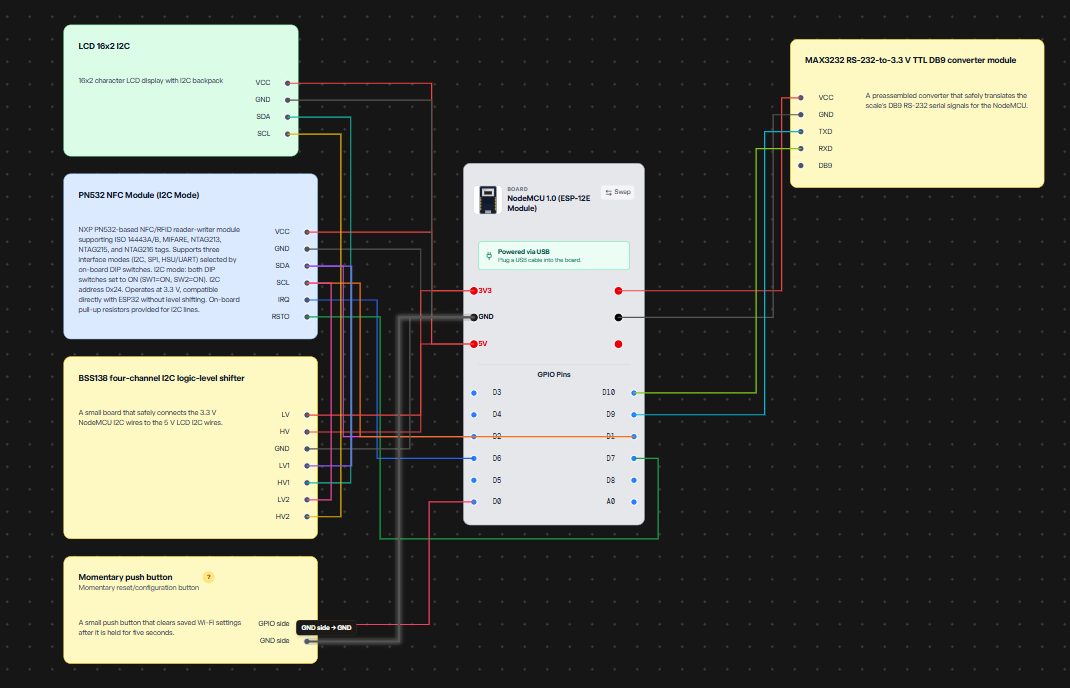
\includegraphics[width=\textwidth]{cablage-prototype.png}
  \caption{Schéma de câblage du module d'acquisition.}
  \label{fig:cablage}
\end{figure}

\begin{table}[H]
\centering
\renewcommand{\arraystretch}{1.2}
\begin{tabular}{|l|l|l|l|}
\hline
\enteteligne \entete{Composant} & \entete{Broche} & \entete{NodeMCU} & \entete{Rôle} \\ \hline
\multirow{4}{*}{MAX3232} & VCC / GND & 3V3 / GND & Alimentation \\
 & TXD & D9 (GPIO3, RX) & Réception des trames de la balance \\
 & RXD & D10 (GPIO1, TX) & Envoi des commandes à la balance \\
 & DB9 & -- & Liaison RS-232 avec la balance \\ \hline
\multirow{4}{*}{PN532} & VCC / GND & 3V3 / GND & Alimentation \\
 & SDA / SCL & D2 / D1 & Bus I$^2$C \\
 & IRQ & D6 & Signal de détection d'un badge \\
 & RSTO & D7 & Réinitialisation du lecteur \\ \hline
\multirow{2}{*}{BSS138} & LV / HV & 3V3 / 5V & Références de tension \\
 & LV1, LV2 / HV1, HV2 & D2, D1 / LCD & Adaptation de SDA et SCL \\ \hline
LCD 16$\times$2 & VCC / GND & 5V / GND & Alimentation \\ \hline
Bouton & GPIO / GND & D0 / GND & Effacement de la configuration Wi-Fi \\ \hline
\end{tabular}
\caption{Connexions du module d'acquisition.}
\label{tab:cablage}
\end{table}

La liaison série croise les signaux : la sortie TXD du MAX3232 est reliée à l'entrée RX du NodeMCU, et son entrée RXD à la sortie TX. Cette liaison utilise l'UART matériel de l'ESP8266, également relié au port USB de programmation : en fonctionnement, il est réservé à la balance, et le programme est téléversé balance débranchée.

\subsection{Protocole de communication avec la balance}

\subsubsection*{Paramètres de la liaison série}

Une liaison \ac{RS-232} ne fonctionne que si les deux extrémités utilisent les mêmes paramètres : débit, nombre de bits de données, parité et bits d'arrêt \citep{tia232}. Le module est configuré selon le paramétrage de l'interface de la balance.
% À VÉRIFIER : remplacer par les paramètres réellement configurés sur la balance.
Nous avons retenu une configuration 9600~bauds, 8~bits de données, sans parité, 1~bit d'arrêt (8N1).

\subsubsection*{Jeu de commandes MT-SICS}

Les balances Mettler Toledo communiquent selon le protocole \ac{MT-SICS} \citep{mtsics}. Le module envoie une commande textuelle terminée par un retour chariot et un saut de ligne, et la balance répond par une trame de même format. Le tableau~\ref{tab:mtsics} présente les commandes utilisées.

\begin{table}[H]
\centering
\renewcommand{\arraystretch}{1.25}
\begin{tabularx}{\textwidth}{|c|Y|l|}
\hline
\enteteligne \entete{Commande} & \entete{Effet} & \entete{Exemple de réponse} \\ \hline
\texttt{S} & Envoie la prochaine valeur de poids \emph{stable} & \texttt{S S \ \ \ \ 100.00 g} \\ \hline
\texttt{SI} & Envoie immédiatement la valeur courante, stable ou non & \texttt{S D \ \ \ \ \ 99.87 g} \\ \hline
\texttt{Z} & Remet la balance à zéro & \texttt{Z A} \\ \hline
\end{tabularx}
\caption{Commandes MT-SICS utilisées par le module.}
\label{tab:mtsics}
\end{table}

Le deuxième champ de la réponse indique l'état de la mesure : \texttt{S} pour une valeur stable, \texttt{D} pour une valeur dynamique (instable), \texttt{I} si la commande ne peut pas être exécutée, \texttt{+} ou \texttt{-} en cas de dépassement de la plage de pesée. Le module n'enregistre comme mesure que les valeurs stables, ce qui garantit que la donnée transmise correspond à une pesée valide.

\subsubsection*{Données mises à disposition}

Le module expose un point d'accès \ac{HTTP}, \texttt{/getData}, que le système d'information interroge pour récupérer la dernière mesure au format \ac{JSON}. Le tableau~\ref{tab:donnees-json} décrit les données transmises.

% À ADAPTER : aligner les noms de champs sur ceux du programme embarqué.
\begin{table}[H]
\centering
\renewcommand{\arraystretch}{1.2}
\begin{tabularx}{\textwidth}{|l|Y|l|}
\hline
\enteteligne \entete{Donnée} & \entete{Description} & \entete{Exemple} \\ \hline
Valeur & Valeur numérique de la pesée & \texttt{100.00} \\ \hline
Unité & Unité renvoyée par la balance & \texttt{g} \\ \hline
Stabilité & État de la mesure (stable ou non) & \texttt{S} \\ \hline
Opérateur & Identifiant du dernier badge NFC lu & \texttt{04A1B2C3} \\ \hline
Horodatage & Instant d'acquisition de la mesure & \texttt{2026-09-23 14:27:20} \\ \hline
\end{tabularx}
\caption{Données transmises par le point d'accès \texttt{/getData}.}
\label{tab:donnees-json}
\end{table}

\subsection{Logique du programme embarqué}

La figure~\ref{fig:organigramme} présente l'organigramme du programme embarqué. Au démarrage, le module initialise ses périphériques et vérifie si le bouton est maintenu pendant cinq secondes, auquel cas il efface la configuration \ac{Wi-Fi}. S'il ne connaît aucun réseau, il ouvre un point d'accès de configuration, qui permet de saisir les identifiants du réseau depuis un téléphone sans reprogrammer le module. Une fois connecté, il affiche son adresse \ac{IP} sur l'écran, puis entre dans sa boucle principale : il mémorise le badge de l'opérateur, traite les trames de la balance et répond aux requêtes du système d'information.

Le module lit l'identifiant du badge et l'associe aux mesures. Le contrôle d'accès par liste de badges autorisés est prévu dans la conception et pourra être activé selon les besoins de Pharmaghreb.

\begin{figure}[H]
\centering
\begin{tikzpicture}[
    decision/.append style={text width=2.0cm, font=\scriptsize},
    bloc/.append style={font=\scriptsize}]
  % Initialisation
  \node[debutfin] (start) at (0,0) {Démarrage};
  \node[bloc=2.8cm] (init) at (0,-1.3) {Initialiser le LCD, le lecteur NFC et l'UART};
  \node[decision] (d1) at (0,-3.0) {Bouton maintenu 5 s ?};
  \node[bloc=2.6cm] (eff) at (3.7,-3.0) {Effacer la configuration Wi-Fi};
  \node[decision] (d2) at (0,-5.2) {Réseau Wi-Fi configuré ?};
  \node[bloc=2.6cm] (ap) at (3.7,-5.2) {Ouvrir le point d'accès de configuration};
  \node[bloc=2.8cm] (cnx) at (0,-7.0) {Se connecter au réseau local};
  \node[bloc=2.8cm] (aff) at (0,-8.3) {Afficher l'état et l'adresse IP};
  % Boucle principale
  \node[decision] (d3) at (9,0) {Badge NFC présenté ?};
  \node[bloc=3.2cm] (a3) at (9,-1.55) {Mémoriser l'identifiant de l'opérateur};
  \node[decision] (d4) at (9,-3.3) {Trame série reçue ?};
  \node[bloc=3.4cm] (a4) at (9,-4.95) {Analyser la trame ; si stable, mémoriser la mesure horodatée et l'afficher};
  \node[decision] (d5) at (9,-6.75) {Requête \texttt{/getData} ?};
  \node[bloc=3.2cm] (a5) at (9,-8.3) {Répondre en JSON};
  \node[font=\scriptsize\bfseries, text=bleu] at (9,1.45) {Boucle principale};

  \draw[fleche] (start) -- (init);
  \draw[fleche] (init) -- (d1);
  \draw[fleche] (d1) -- node[above, etiq] {oui} (eff);
  \draw[fleche] (d1) -- node[right, etiq] {non} (d2);
  \draw[fleche] (eff.south) |- (0,-4.15);
  \draw[fleche] (d2) -- node[above, etiq] {non} (ap);
  \draw[fleche] (d2) -- node[right, etiq] {oui} (cnx);
  \draw[fleche] (ap) |- (cnx);
  \draw[fleche] (cnx) -- (aff);
  \draw[fleche] (aff.east) -- (6.3,-8.3) |- (9,1.0) -- (d3);

  \draw[fleche] (d3) -- node[right, etiq] {oui} (a3);
  \draw[fleche] (a3) -- (d4);
  \draw[fleche] (d3.west) -- node[above, etiq] {non} (7.1,0) |- (9,-2.45);
  \draw[fleche] (d4) -- node[right, etiq] {oui} (a4);
  \draw[fleche] (a4) -- (d5);
  \draw[fleche] (d4.west) -- node[above, etiq] {non} (7.1,-3.3) |- (9,-5.85);
  \draw[fleche] (d5) -- node[right, etiq] {oui} (a5);
  \draw[fleche] (d5.east) -- node[above, etiq] {non} (11.6,-6.75) |- (9,1.0);
  \draw[fleche] (a5.east) -| (11.6,-6.75);
\end{tikzpicture}
\caption{Organigramme du programme embarqué du module d'acquisition.}
\label{fig:organigramme}
\end{figure}

%-------------------------------------------------------------
\section*{Conclusion}
\addcontentsline{toc}{section}{Conclusion}
%-------------------------------------------------------------

Ce chapitre a présenté la conception des deux solutions. Le module de traçabilité repose sur une architecture en trois niveaux, un algorithme d'identification des codes fondé sur leur structure et un modèle de données qui relie demandes, échantillons, réceptions, lots, préparations et opérations. Le module d'acquisition repose sur un microcontrôleur ESP8266 qui dialogue avec la balance selon le protocole \ac{MT-SICS}, identifie l'opérateur par badge \ac{NFC} et met les mesures à disposition par \ac{Wi-Fi}. Le chapitre suivant présente la réalisation de ces deux solutions.
